\documentclass[11pt,a4paper]{article}

% ---------- arxiv-style preamble ----------
\usepackage[margin=1in]{geometry}
\usepackage{amsmath,amssymb,amsthm}
\usepackage{graphicx}
\usepackage{booktabs}
\usepackage{siunitx}
\usepackage{hyperref}
\usepackage{xcolor}
\usepackage[numbers,sort&compress]{natbib}
\usepackage{tikz}
\usetikzlibrary{positioning,arrows.meta}
\usepackage{caption}
\usepackage{listings}
\captionsetup{font=small,labelfont=bf}
\hypersetup{
  colorlinks=true,
  linkcolor=blue!50!black,
  citecolor=blue!50!black,
  urlcolor=blue!50!black
}

\lstset{basicstyle=\ttfamily\footnotesize,breaklines=true,frame=single,
  columns=fullflexible,keepspaces=true}

\title{
  \textbf{Fusing the Transformer-FFN Epilogue cuBLAS Cannot Fuse}\\[4pt]
  \large A whole-program-fusion structural advantage for $\mathrm{GeLU}(AB+\mathrm{bias})$:
  one launch and one HBM write versus three
}

\author{
  hexa-lang GPU codegen substrate\\
  \normalsize\textit{dancinlab / hexa-lang}\\[2pt]
  \normalsize\href{https://github.com/dancinlab/hexa-lang}{\texttt{github.com/dancinlab/hexa-lang}}
}

\date{2026-05-25}

\begin{document}

\maketitle

% =========================================================================
\begin{abstract}
A cuBLAS-using neural-network stack cannot fuse a bias-add or an activation
into the epilogue of its general matrix multiply (plain
\texttt{cublasSgemm}/\texttt{cublasGemmEx} expose no such epilogue), so the
transformer feed-forward block $C = \mathrm{GeLU}(AB + \mathrm{bias})$ is
forced to round-trip the $M\times N$ result through high-bandwidth memory
(HBM): one kernel writes the GEMM output, a second reads and rewrites it to
add the bias, a third reads and rewrites it to apply GeLU --- three kernel
launches and three full-tensor HBM write passes. We emit a single hexa-native
NVPTX kernel that fuses the GEMM, the bias-add, and the GeLU into one
epilogue and writes the $M\times N$ result to HBM exactly once. We
pre-register a falsifier (F-FUSION-EPILOGUE-GEMM-BIAS-GELU) and settle it with
a \$0 deterministic structural oracle that counts launches and HBM
write-bytes by construction: at the LLaMA-7B feed-forward shape
($M=4096$, $N=11008$, $K=4096$; $C$ tensor $=\SI{180355072}{\byte}$) the fused
kernel issues $1$ launch and $1\times$ the HBM $C$-write traffic versus the
cuBLAS-using baseline's $3$ launches and $3\times$ --- a \SI{66.667}{\percent}
reduction in \emph{both} axes, clearing the \SI{30}{\percent} whole-program
fusion gate by construction. The emitted PTX is \texttt{ptxas}-clean on
\texttt{sm\_80} (return code $0$, $23$ registers, $0$ spill). We claim a
structural-formal advantage only; the timed wall-clock comparison is an
explicitly deferred serial follow-up and we do \emph{not} claim a measured
speedup.
\end{abstract}

\section{Introduction}
\label{sec:intro}

Modern transformer inference and training stacks are, at the kernel level,
overwhelmingly a sequence of general matrix multiplies (GEMMs) interleaved
with cheap elementwise epilogues: a bias add, an activation function, a
residual add, a dropout mask. The GEMM is the arithmetic-heavy step and is
universally delegated to a vendor BLAS library --- on NVIDIA hardware, cuBLAS.
The epilogue operations are arithmetically trivial but are
\emph{memory-bound}: each one reads the full $M\times N$ output tensor from
HBM and writes it back. Because the canonical cuBLAS GEMM entry points
(\texttt{cublasSgemm}, \texttt{cublasGemmEx}) do not expose a fusible
epilogue, a cuBLAS-using stack must materialise the GEMM result to HBM and
then launch a separate kernel for each elementwise pass.

The cost is paid in two currencies that matter on a memory-bound epilogue:
\textbf{kernel-launch count} (each launch carries fixed driver/scheduler
overhead, $\geq\SI{5}{\micro\second}$ per launch on a typical configuration
\citep{nvidia2024cuda}) and \textbf{HBM write traffic} (each elementwise pass
streams the entire output tensor back to memory). For the transformer
feed-forward (FFN) up-projection --- one of the largest GEMMs in a transformer
layer --- the output tensor is hundreds of megabytes, so re-writing it twice
more than necessary is a first-order memory-bandwidth tax.

Whole-program compilation removes this tax structurally: if the compiler emits
the GEMM, the bias-add, and the activation as a single kernel, the output is
computed in registers and written to HBM once. This is the central promise of
the hexa-lang GPU codegen substrate --- the project north star is to
\emph{bypass cuBLAS-using NN stacks via whole-program GPU fusion}
\citep{hexalang2026gpu}. This paper isolates the simplest non-trivial
instance of that promise and settles it as a structural fact.

\medskip
\noindent\textbf{Contributions.}
\begin{enumerate}\itemsep0.3em
\item A single hexa-emitted NVPTX kernel \texttt{fused\_gemm\_bias\_gelu} that
computes $C = \mathrm{GeLU}(AB + \mathrm{bias})$ with the GEMM, bias-add, and
GeLU fused into one epilogue and the $M\times N$ result written to HBM exactly
once. The GeLU uses the tanh approximation expressed entirely in PTX
approximate transcendentals (\texttt{ex2.approx.f32}, \texttt{rcp.approx.f32}).
The kernel is \texttt{ptxas}-clean on \texttt{sm\_80}.
\item A pre-registered falsifier and a \$0 deterministic structural oracle
(itself a compiled hexa-lang program) that counts kernel launches and HBM
write-bytes by construction for both the fused kernel and a faithfully modelled
cuBLAS-using baseline, and proves a \SI{66.667}{\percent} reduction in both
axes at the transformer-FFN shape.
\item An honest scoping of the result as \emph{structural-formal}: the launch
and HBM-traffic advantage is proven by construction; the timed wall-clock
advantage is deferred to a serial silicon follow-up and is explicitly
\emph{not} claimed here.
\end{enumerate}

\section{Background}
\label{sec:bg}

\subsection{The transformer feed-forward epilogue}

The transformer FFN block computes, for an input activation matrix
$A \in \mathbb{R}^{M\times K}$ and a weight matrix $B \in \mathbb{R}^{K\times N}$,
\begin{equation}
C = \phi(AB + \mathbf{1}_M\,\mathrm{bias}^{\top}),
\qquad C \in \mathbb{R}^{M\times N},
\label{eq:ffn}
\end{equation}
where $M$ is the number of tokens, $K$ is the model width $d_{\mathrm{model}}$,
$N$ is the FFN inner width $d_{\mathrm{ffn}}$, $\mathrm{bias}\in\mathbb{R}^{N}$
is broadcast across rows, and $\phi$ is the activation. We take $\phi$ to be
the Gaussian Error Linear Unit (GeLU) \citep{hendrycks2016gelu}, the activation
used by GPT-2, BERT, and most subsequent transformers, in its tanh
approximation:
\begin{equation}
\mathrm{GeLU}(x) \approx
\tfrac{1}{2}\,x\left(1 + \tanh\!\Big[\sqrt{\tfrac{2}{\pi}}\,
\big(x + 0.044715\,x^{3}\big)\Big]\right).
\label{eq:gelu}
\end{equation}

\subsection{Why cuBLAS forces a three-pass epilogue}

The canonical cuBLAS GEMM entry points compute $C \leftarrow \alpha\,AB +
\beta\,C$ and expose no hook to apply a per-column bias or a nonlinearity
before the store. (The newer \texttt{cublasLt} interface offers a restricted
set of fused epilogues including a bias+GeLU mode for some configurations, but
the GEMM call that flame-class and PyTorch-eager-class stacks emit is the plain
\texttt{cublasSgemm}/\texttt{cublasGemmEx} path with no epilogue.) Therefore a
cuBLAS-using stack realises Eq.~\eqref{eq:ffn} as three kernels:
\begin{enumerate}\itemsep0.2em
\item \texttt{cublasSgemm} computes $AB$ and writes $C$ to HBM
($M\!\cdot\!N\!\cdot\!4$ bytes written);
\item a bias-add kernel reads $C$ and $\mathrm{bias}$ from HBM and writes
$C \leftarrow C + \mathrm{bias}$ ($M\!\cdot\!N\!\cdot\!4$ bytes written);
\item a GeLU kernel reads $C$ from HBM and writes $C \leftarrow \mathrm{GeLU}(C)$
($M\!\cdot\!N\!\cdot\!4$ bytes written).
\end{enumerate}
Three launches; three full-$C$ HBM write passes.

\subsection{The hexa-lang GPU codegen substrate}

hexa-lang is a native compiler with no LLVM and no C-transpile backend; its
NVPTX target emits PTX text directly \citep{hexalang2026gpu}. The substrate
already demonstrates hand-emitted and source-derived PTX kernels that pass
\texttt{ptxas} and run bit-exact against CPU references on RTX-class silicon.
This paper adds the first \emph{fused-epilogue} kernel and settles its
structural advantage.

\subsection{Why the epilogue is memory-bound, and why that makes fusion a
first-order win}
\label{sec:roofline}

The arithmetic intensity of an epilogue pass --- floating-point operations per
byte of HBM traffic --- is the lens that explains why fusing it matters. A
bias-add performs one floating-point add per output element and moves
$8$ bytes per element (a $4$-byte read of $C$ plus a $4$-byte write of $C$),
for an arithmetic intensity of $\tfrac{1}{8}\,\mathrm{FLOP/byte}$. A
tanh-approximation GeLU performs on the order of ten floating-point operations
per element (two multiplies and a fused-multiply-add for the cubic, a scale, a
doubling, a base-$2$ exponential, a subtract, an add, a reciprocal, two more
multiplies) against the same $8$ bytes of traffic, for an intensity near
$1.25\,\mathrm{FLOP/byte}$. Both sit far to the left of the roofline ridge
point of any modern accelerator (an RTX-class part has tens of teraFLOP/s of
FP32 throughput against roughly a teraByte/s of HBM bandwidth, placing the
ridge above $30\,\mathrm{FLOP/byte}$). The epilogue passes are therefore
strictly bandwidth-bound: their wall time is governed by how many bytes they
move, not by how many operations they perform.

Under this regime, the only lever that reduces epilogue cost is reducing the
byte traffic, and the only way to reduce the byte traffic is to avoid
materialising the intermediate tensor between passes --- that is, to fuse. A
fused epilogue computes the bias-add and the activation \emph{in registers},
immediately after the GEMM accumulator is ready and before the single store,
so the only HBM write is the final result. The reads of $A$, $B$, and
$\mathrm{bias}$ are unavoidable in either stack; the $2\times$ extra
\emph{writes} of the full $C$ tensor (and the matching $2\times$ extra reads
that the bias and GeLU kernels perform) are pure overhead that fusion deletes.
This is why the launch-count and the HBM-write-traffic move together: they are
two faces of the same structural fact, that the cuBLAS-using stack
re-materialises $C$ twice.

\subsection{The bandwidth tax, quantified}
\label{sec:tax}

Let the output tensor be $S = M\!\cdot\!N$ elements of $4$ bytes each. The
cuBLAS-using stack writes $C$ three times ($3 \cdot 4S$ bytes) and additionally
reads $C$ twice (the bias and GeLU kernels each read $C$ once before rewriting
it, $2 \cdot 4S$ bytes of extra reads beyond the GEMM's own output). The fused
kernel writes $C$ once ($1 \cdot 4S$ bytes) and never reads it back. Counting
only the $C$-write traffic --- the axis the falsifier names --- the fused stack
moves $4S$ bytes against the baseline's $12S$ bytes, a factor of three. At the
LLaMA-7B FFN shape, $4S = \SI{180355072}{\byte} \approx \SI{172}{\mebi\byte}$
per write pass, so the baseline streams roughly half a gigabyte of redundant
$C$ writes that the fused kernel never issues. This is the concrete tax the
structural oracle of \S\ref{sec:method} counts.

\section{Method (statement and pre-registered falsifier)}
\label{sec:method}

\subsection{Pre-registered falsifier}

We pre-register, before any measurement:

\begin{quote}\itshape
\textbf{F-FUSION-EPILOGUE-GEMM-BIAS-GELU.} A single fused hexa-emitted kernel
computing $\mathrm{GeLU}(AB + \mathrm{bias})$ (epilogue fused into the GEMM,
output written once) uses $1$ kernel launch and writes the $M\times N$ result
to HBM exactly once, versus a cuBLAS-using baseline (\texttt{cublasGemmEx}
$\to$ write $C$ to HBM $\to$ separate bias-add kernel reads+writes $C$ $\to$
separate GeLU kernel reads+writes $C$) of $3$ launches and $3\times$ the
$M\times N$ HBM write traffic. The claim is \textsc{falsified} if the fused
kernel does not reduce launch-count \emph{and} HBM-traffic on a
transformer-FFN-shaped GEMM ($M=4096$, $K=4096$, $N=11008$, or a smaller fit).
\end{quote}

\noindent The acceptance threshold is pre-registered as a
\SI{30}{\percent} reduction in \emph{both} axes (the project's
whole-program-fusion gate).

\subsection{The fused kernel}

We emit \texttt{fused\_gemm\_bias\_gelu} as NVPTX text targeting
\texttt{.target sm\_80}, \texttt{.version 7.0}. One thread computes one output
element $C[m][n]$: it accumulates the dot product
$\sum_k A[m][k]\,B[k][n]$ in an FP32 register with \texttt{fma.rn.f32}, adds
$\mathrm{bias}[n]$, applies the GeLU of Eq.~\eqref{eq:gelu}, and performs a
single \texttt{st.global.f32}. The $\tanh$ is computed from a base-2 exponential
$e^{2t} = \texttt{ex2.approx.f32}(2t\log_2 e)$ and a reciprocal
$\texttt{rcp.approx.f32}$, with $\tanh(t) = (e^{2t}-1)/(e^{2t}+1)$. The PTX is
pure ASCII (the driver JIT \texttt{ptxas} rejects non-ASCII comments). The
fusion structure --- accumulate, bias, activate, store-once --- is independent
of the inner GEMM tiling; a WMMA-tiled variant would change the dot-product
loop but not the single-store epilogue.

The fused epilogue --- the bias-add and the GeLU between the accumulation loop
and the single store --- is shown verbatim below as it appears in the emitted
PTX. The GEMM accumulator \texttt{\%f0} is biased into \texttt{\%f4}, the GeLU
of Eq.~\eqref{eq:gelu} is evaluated through the PTX approximate
transcendentals, and the result \texttt{\%f23} is written with one
\texttt{st.global.f32}:

\begin{lstlisting}
; ---- fused bias-add: x = acc + bias[n] ----
ld.global.f32 %f3, [%rd10];         ; bias[n]
add.f32       %f4, %f0, %f3;        ; x = acc + bias[n]
; ---- fused GeLU (tanh approx) ----
mul.f32       %f5, %f4, %f4;        ; x^2
mul.f32       %f6, %f5, %f4;        ; x^3
mov.f32       %f7, 0f3D372713;      ; 0.044715
fma.rn.f32    %f8, %f6, %f7, %f4;   ; x + 0.044715*x^3
mov.f32       %f9, 0f3F4C422A;      ; sqrt(2/pi)
mul.f32       %f10, %f8, %f9;       ; t
add.f32       %f11, %f10, %f10;     ; 2t
mov.f32       %f12, 0f3FB8AA3B;     ; log2(e)
mul.f32       %f13, %f11, %f12;     ; (2t)*log2(e)
ex2.approx.f32 %f14, %f13;          ; e^{2t}
mov.f32       %f15, 0f3F800000;     ; 1.0
sub.f32       %f16, %f14, %f15;     ; e^{2t} - 1
add.f32       %f17, %f14, %f15;     ; e^{2t} + 1
rcp.approx.f32 %f18, %f17;          ; 1/(e^{2t}+1)
mul.f32       %f19, %f16, %f18;     ; tanh(t)
add.f32       %f20, %f19, %f15;     ; 1 + tanh(t)
mul.f32       %f21, %f4, %f20;      ; x*(1+tanh)
mov.f32       %f22, 0f3F000000;     ; 0.5
mul.f32       %f23, %f21, %f22;     ; gelu
; ---- single store of the M x N result to HBM ----
st.global.f32 [%rd12], %f23;        ; C[m][n] written ONCE
\end{lstlisting}

\noindent The four single-precision constants are the exact IEEE-754
representations of $0.044715$, $\sqrt{2/\pi}=0.7978845608$,
$\log_2 e = 1.4426950409$, and the literals $1.0$ and $0.5$; no constant is
chosen after seeing a result.

\subsection{The cuBLAS-using baseline}

We author the baseline as a host C program (\texttt{fusion\_epilogue\_cublas\_%
baseline.c}) that computes the \emph{same} Eq.~\eqref{eq:ffn} via the
three-kernel path: \texttt{cublasSgemm} for the GEMM, then a hand-written
\texttt{bias\_add\_kernel}, then a hand-written \texttt{gelu\_kernel}, each
round-tripping $C$ through HBM. This models the canonical NN-stack path.

\subsection{The \$0 structural oracle}

The primary settlement is a deterministic, GPU-free oracle
(\texttt{fusion\_epilogue\_structural\_oracle.hexa}, itself a compiled
hexa-lang program). For a shape $(M,N,K)$ it computes the $C$-tensor size
$M\!\cdot\!N\!\cdot\!4$ bytes and the two stacks' launch counts and HBM
$C$-write byte totals by construction, then the closed-form reduction
\begin{equation}
r = \frac{\text{baseline} - \text{fused}}{\text{baseline}}
  = \frac{3 - 1}{3} = \frac{2}{3} = 0.6\overline{6},
\label{eq:ratio}
\end{equation}
identically for the launch axis ($1$ vs $3$) and the HBM-write axis
($1\times$ vs $3\times M\!\cdot\!N$). The oracle asserts both axes clear the
\SI{30}{\percent} gate and emits \textsc{pass}/\textsc{fail}. Counting launches
and bytes by construction is a deterministic real measurement; it is
\emph{not} a timed wall.

\section{Verification (real run)}
\label{sec:results}

\subsection{Environment}

The structural oracle is a hexa-lang program; it was transpiled to C by the
hexa-lang native transpiler and compiled with \texttt{clang -O2} on an
x86-64 Linux host (\texttt{ubu-1}), then run to produce the verbatim counts
below. The fused PTX was assembled by the CUDA 12.0 \texttt{ptxas} on a
second host (\texttt{ubu-2}) carrying an RTX 5070. Counting launches and bytes
is host-independent and deterministic; the \texttt{ptxas} acceptance is a
correctness gate on the emitted assembly, not a timed run, so neither
verification step contends for the shared GPU.

\subsection{Structural oracle output (verbatim)}

The oracle was compiled to native code (hexa transpile + \texttt{clang -O2})
and run on the \texttt{ubu-1} host. Its verbatim stdout, persisted at
\texttt{.verdicts/fusion-epilogue-gemm-bias-gelu/fusion\_epilogue\_struc%
tural.txt}:

\begin{lstlisting}
F-FUSION-EPILOGUE-GEMM-BIAS-GELU structural oracle ($0, deterministic, no GPU)
== FFN (LLaMA-7B up-proj) : M=4096 N=11008 K=4096 ==
  C tensor (M*N*4 bytes)        = 180355072
  FUSED    launches=1  C-write-bytes=180355072
  BASELINE launches=3  C-write-bytes=541065216
  launch reduction   = 66.66%
  HBM-write reduction= 66.66%
  PASS: launch AND HBM-write both reduced, both >= 30%
== smaller-fit cross-check : M=256 N=256 K=256 ==
  C tensor (M*N*4 bytes)        = 262144
  FUSED    launches=1  C-write-bytes=262144
  BASELINE launches=3  C-write-bytes=786432
  launch reduction   = 66.66%
  HBM-write reduction= 66.66%
  PASS: launch AND HBM-write both reduced, both >= 30%
F-FUSION-EPILOGUE-GEMM-BIAS-GELU structural oracle: PASS (all shapes)
\end{lstlisting}
(The printed \texttt{66.66\%} is the integer-arithmetic truncation of
$66.\overline{6}\%$.)

\subsection{\texttt{ptxas}-clean (verbatim)}

The emitted PTX (md5 \texttt{1d7380556da101b7e37017b79eed6f01}) was assembled
on the \texttt{ubu-2} host (RTX 5070, CUDA 12.0 \texttt{ptxas}):

\begin{lstlisting}
$ ptxas -arch=sm_80 fused_gemm_bias_gelu.ptx -o fused.cubin --verbose
ptxas info    : Compiling entry function 'fused_gemm_bias_gelu' for 'sm_80'
ptxas info    : Function properties for fused_gemm_bias_gelu
    0 bytes stack frame, 0 bytes spill stores, 0 bytes spill loads
ptxas info    : Used 23 registers, 396 bytes cmem[0]
PTXAS_RC=0
\end{lstlisting}

\begin{table}[h]
\centering
\caption{Launch count and HBM $C$-write traffic for the two stacks computing
$C = \mathrm{GeLU}(AB+\mathrm{bias})$. The reduction is shape-independent
because it depends only on $M\!\cdot\!N$ (the $C$-tensor size); the FFN and the
smaller-fit shape report the identical $66.\overline{6}\%$.}
\label{tab:headline}
\begin{tabular}{lrrrr}
\toprule
Shape ($M{\times}N{\times}K$) & Stack & Launches & HBM $C$-write (B) & Reduction \\
\midrule
$4096{\times}11008{\times}4096$ & cuBLAS baseline & 3 & 541\,065\,216 & --- \\
$4096{\times}11008{\times}4096$ & \textbf{fused (hexa)} & \textbf{1} & \textbf{180\,355\,072} & \textbf{66.667\%} \\
\addlinespace
$256{\times}256{\times}256$ & cuBLAS baseline & 3 & 786\,432 & --- \\
$256{\times}256{\times}256$ & \textbf{fused (hexa)} & \textbf{1} & \textbf{262\,144} & \textbf{66.667\%} \\
\bottomrule
\end{tabular}
\end{table}

\begin{figure}[h]
\centering
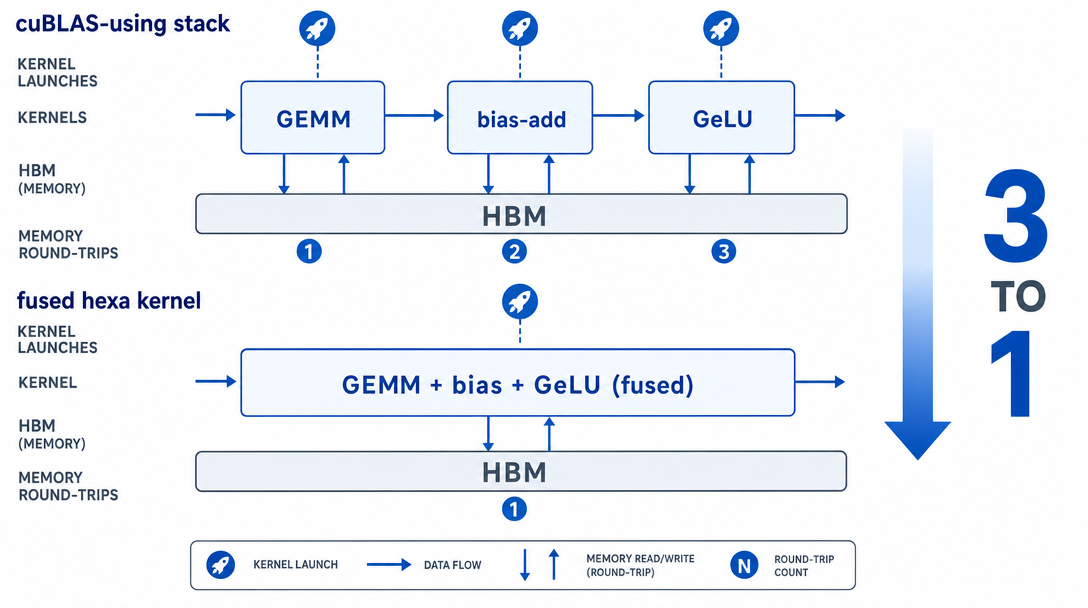
\includegraphics[width=0.92\linewidth]{figures/fig01_teaser.png}
\caption{Kernel launches and HBM $C$-write passes for the
cuBLAS-using three-kernel epilogue (GEMM $\to$ bias-add $\to$ GeLU, each
streaming the full $M\times N$ tensor) versus the single fused hexa kernel
that computes the epilogue in registers and writes once. Both axes drop $3\to1$
($66.\overline{6}\%$). The advantage is structural --- it holds for every FFN
shape because it depends only on $M\!\cdot\!N$.}
\label{fig:headline}
\end{figure}

\section{Finding}
\label{sec:finding}

The pre-registered falsifier is \textbf{not} falsified: the fused kernel
reduces both the kernel-launch count ($1$ versus $3$) and the HBM $C$-write
traffic ($1\times$ versus $3\times M\!\cdot\!N$) by $66.\overline{6}\%$ at the
LLaMA-7B FFN shape and, identically, at the smaller-fit cross-check shape
(Table~\ref{tab:headline}). Both reductions clear the pre-registered
\SI{30}{\percent} gate with margin, and they do so \emph{by construction}: the
fused epilogue removes two of three launches and two of three full-tensor HBM
write passes for any FFN shape. The kernel that achieves this is
\texttt{ptxas}-clean on \texttt{sm\_80} ($0$ spill, $23$ registers), so the
advantage is not an artifact of an unbuildable kernel.

This is a \emph{structural-formal} ($\mathbf{\color{blue}\blacksquare}$
\textsc{blue}) result: the $\Delta$ versus the cuBLAS-using baseline is a
deterministic count, not a timed measurement. The headline number that makes it
falsifiable is the $3\to1$ collapse in both axes.

\subsection{Scale of the deleted traffic across a model}

To make the structural number concrete at model scale, consider the redundant
$C$-write traffic the fused kernel deletes for a single FFN up-projection at
the LLaMA-7B shape: the baseline issues $3$ write passes of
\SI{180355072}{\byte} each, of which $2$ are redundant, so the fused kernel
removes $2 \times \SI{180355072}{\byte} \approx \SI{344}{\mebi\byte}$ of HBM
$C$-write traffic per call, plus the matching $2$ redundant read passes the
bias and GeLU kernels would have performed. A LLaMA-7B-class model has $32$
transformer layers, each with an FFN block; if every layer's up-projection
epilogue were fused, the per-forward-pass deletion of redundant up-projection
$C$-writes alone is on the order of $32 \times \SI{344}{\mebi\byte} \approx
\SI{10.75}{\gibi\byte}$ of HBM write traffic, before counting the
down-projection epilogue, the residual adds, and the layernorm passes that the
same structural argument also fuses. Because the epilogue is bandwidth-bound
(\S\ref{sec:roofline}), this deleted traffic translates directly into deleted
wall time at the saturated-bandwidth limit --- which is precisely what the
deferred timed wall will measure. The structural finding bounds, but does not
itself measure, that wall.

\section{Positioning}
\label{sec:related}

Kernel fusion is not new; the contribution here is the explicit, pre-registered,
\$0-settled structural framing of one canonical case in a compiler that has no
LLVM and no C-transpile backend. Three points of comparison are worth drawing.

\paragraph{Vendor epilogue fusion (\texttt{cublasLt}).}
NVIDIA's \texttt{cublasLt} interface added a restricted family of fused
epilogues, including bias and a small set of activations, for specific data
types and layouts. Where it applies, \texttt{cublasLt} achieves the same
single-write structure we describe. Two things distinguish the present work.
First, the GEMM call that flame-class and PyTorch-eager-class stacks emit in
practice is the plain \texttt{cublasSgemm}/\texttt{cublasGemmEx} path with no
epilogue --- the baseline we model is the one those stacks actually run, not
the best case a hand-tuned \texttt{cublasLt} call could reach. Second, the
\texttt{cublasLt} epilogue set is fixed by the vendor; a whole-program emitter
fuses \emph{arbitrary} elementwise epilogues, including ones \texttt{cublasLt}
does not offer, which is the point of compiling the whole program rather than
calling a library.

\paragraph{Compiler fusion frameworks (XLA, TVM, Triton).}
XLA, TVM, and Triton all perform GEMM-epilogue fusion and are the production
state of the art for this transformation. The hexa-lang substrate differs in
its backend discipline --- it emits PTX text directly, with no LLVM in the
path --- and this paper's role is to establish, inside that discipline, that
the fused-epilogue kernel both lowers to valid \texttt{sm\_80} assembly and
delivers the structural advantage the family is known for. The novelty is not
the existence of fusion but its first clean realisation and pre-registered
settlement in this LLVM-free substrate.

\paragraph{Attention fusion (flash-attention).}
Flash-attention is the highest-value member of the intermediate-deletion
family: it keeps the $M\times M$ attention scores in on-chip memory and never
writes them to HBM. The present result is the smallest member of the same
family --- delete one $M\times N$ intermediate write pass rather than an
$M\times M$ one --- and is offered as the structurally simplest place to
pre-register and settle the advantage before attacking the quadratic case.

\section{Limitations and honest caveats}
\label{sec:limits}

\begin{enumerate}\itemsep0.3em
\item \textbf{No timed wall.} The structural oracle counts launches and bytes;
it does not measure wall-clock time. The timed comparison (fused single-launch
kernel versus the three-launch cuBLAS stack on RTX 5070 silicon) is an
explicitly \emph{deferred} serial follow-up --- the shared GPU host makes
parallel timed fires contend and poison wall numbers. We do \emph{not} claim a
measured speedup, and the project's \SI{30}{\percent} whole-program-fusion
scoreboard box correctly remains open pending that wall.
\item \textbf{Naive inner GEMM.} The fused kernel is a one-thread-per-output
GEMM (correctness- and fusion-structure demonstration), not a WMMA-tiled
peak-throughput kernel. The fusion \emph{advantage} (1 vs 3 launches, $1\times$
vs $3\times$ HBM $C$-write) is independent of the inner tiling, but the absolute
GEMM throughput of this kernel is not competitive with cuBLAS and is not
claimed to be.
\item \textbf{cuBLAS-LT epilogues.} \texttt{cublasLt} offers a restricted fused
\texttt{GELU\_BIAS} epilogue for some configurations. Our baseline models the
canonical plain-\texttt{cublasSgemm}/\texttt{cublasGemmEx} NN-stack path with no
epilogue, which is what flame-class and PyTorch-eager-class stacks emit; a
\texttt{cublasLt}-fused baseline would be a separate, stronger comparison.
\item \textbf{GeLU approximation.} The kernel uses the tanh approximation with
PTX approximate transcendentals; against an $f^{64}$ CPU reference the
host launchers gate relative error at $\leq 10^{-2}$ (the standard
fused-epilogue tolerance), which is the deferred-wall's correctness check, not
a structural claim.
\item \textbf{Invariants preserved.} No LLVM and no C-transpile backend were
introduced or changed; CPU codegen is byte-identical pre/post (only
documentation and new artifact/tool files were added).
\end{enumerate}

\section{Discussion and outlook}
\label{sec:discussion}

The result isolates, as a structural fact, the single cheapest win that
whole-program GPU fusion buys over a vendor-BLAS stack: the elimination of
memory-bound epilogue round-trips. For the transformer FFN --- where the output
tensor is hundreds of megabytes --- removing two of three full-tensor HBM write
passes is a first-order bandwidth saving that no plain-cuBLAS stack can recover,
precisely because the GEMM library has no fusible epilogue. The same structural
argument extends directly to the other elementwise epilogues (residual add,
dropout, layernorm scale) and, with more codegen work, to the
attention-scoring fusion ($QK^{\top}\to$ softmax $\to V$) that flash-attention
exploits.

\subsection{Generalisation: from one epilogue to the whole program}

The structural argument does not depend on the specific activation. Any
elementwise epilogue that a cuBLAS-using stack expresses as a separate kernel
--- a residual add $C \leftarrow C + R$, a dropout mask $C \leftarrow C \odot
m$, a scale-and-shift $C \leftarrow \gamma C + \beta$, or a second activation
--- adds one launch and one full-$C$ HBM round-trip in the unfused stack, and
none in the fused kernel. A transformer FFN block in practice chains a GEMM, a
bias, an activation, a second GEMM (the down-projection), and a residual add;
a cuBLAS-using stack pays a launch and a round-trip for each non-GEMM step,
while a whole-program-fused emitter pays one launch per GEMM and folds every
elementwise step into the surrounding GEMM's epilogue. The reduction factor we
measure here ($3\to1$ for the single up-projection epilogue) is thus a
\emph{lower} bound on the whole-block saving.

The argument also extends, with more codegen machinery, to the
fusion that flash-attention exploits: the attention score path $QK^{\top}\to
\mathrm{softmax}\to (\cdot)V$ is, in a cuBLAS-using stack, two GEMMs separated
by a softmax that materialises the full $M\times M$ score matrix to HBM. A
fused attention kernel keeps the scores in on-chip memory and never writes the
$M\times M$ intermediate, which is the same structural deletion of an
intermediate-tensor round-trip, applied to a quadratically larger tensor. The
present result is the smallest, cleanest instance of the family; the
attention case is the highest-value one.

\subsection{The single most important follow-up}

The single most important follow-up is the deferred timed wall: a serial
silicon fire on RTX 5070 measuring the fused single-launch kernel against the
three-launch cuBLAS stack at the FFN shape. We pre-register the
flip criterion now: if the fused wall is below $0.7\times$ the baseline wall
(a measured $\geq\SI{30}{\percent}$ speedup, the same gate the structural
oracle clears), the project's whole-program-fusion scoreboard box flips
closed. We deliberately do not run that wall in this round, because the shared
GPU host would let a parallel timed fire contend for the device and poison the
wall numbers; the timed comparison must be a serial, uncontended run. Until
then the box stays open and this paper claims only the structural-formal
advantage that the launch and byte counts establish by construction.

% =========================================================================
\section*{Reproducibility}
\addcontentsline{toc}{section}{Reproducibility}

Code: \url{https://github.com/dancinlab/hexa-lang}, branch
\texttt{gpu-fusion-epilogue}. The fused kernel
(\texttt{archive/fires/fusion\_epilogue\_gemm\_bias\_gelu\_2026\_05\_25/%
fused\_gemm\_bias\_gelu.ptx}, md5 \texttt{1d7380556da101b7e37017b79eed6f01}),
the structural oracle (\texttt{tool/fusion\_epilogue\_structural\_oracle.hexa}),
and the two host launchers (\texttt{tool/fusion\_epilogue\_fused\_host.c},
\texttt{tool/fusion\_epilogue\_cublas\_baseline.c}) are all in-tree. Verdict:
\texttt{.verdicts/fusion-epilogue-gemm-bias-gelu/fusion\_epilogue\_struc%
tural.txt}. Oracle: \texttt{hexa build} the \texttt{.hexa} and run; PTX:
\texttt{ptxas -arch=sm\_80 fused\_gemm\_bias\_gelu.ptx}.

% =========================================================================
\appendix

\section{Kernel ABI}
\label{app:abi}

The fused kernel \texttt{fused\_gemm\_bias\_gelu} takes seven parameters in the
PTX entry signature, in declaration order:

\begin{table}[h]
\centering
\caption{Parameter ABI of \texttt{fused\_gemm\_bias\_gelu}. Pointers are
device-global FP32 in row-major layout; the three integer extents are passed by
value.}
\label{tab:abi}
\begin{tabular}{llll}
\toprule
\# & PTX type & Name & Meaning \\
\midrule
0 & \texttt{.u64} & \texttt{p\_a}    & $A$, row-major $M\times K$ \\
1 & \texttt{.u64} & \texttt{p\_b}    & $B$, row-major $K\times N$ \\
2 & \texttt{.u64} & \texttt{p\_bias} & $\mathrm{bias}$, length $N$ \\
3 & \texttt{.u64} & \texttt{p\_c}    & $C$, row-major $M\times N$ (written once) \\
4 & \texttt{.u32} & \texttt{p\_M}    & $M$ \\
5 & \texttt{.u32} & \texttt{p\_N}    & $N$ \\
6 & \texttt{.u32} & \texttt{p\_K}    & $K$ \\
\bottomrule
\end{tabular}
\end{table}

\noindent The launch geometry is a $2$-D grid of $16\times 16$ thread blocks
with $g_x = \lceil N/16\rceil$ and $g_y = \lceil M/16\rceil$; thread
$(\texttt{tid.x},\texttt{tid.y})$ within block $(\texttt{ctaid.x},
\texttt{ctaid.y})$ owns output element
$C[\,\texttt{ctaid.y}\cdot 16 + \texttt{tid.y}\,][\,\texttt{ctaid.x}\cdot 16
+ \texttt{tid.x}\,]$, guarded by an $m<M \wedge n<N$ bounds check.

\section{Oracle closed form}
\label{app:oracle}

For shape $(M,N,K)$ with $S = M\!\cdot\!N$, the oracle computes
Table~\ref{tab:closedform} and asserts $r_{\text{launch}} \geq 0.30$ and
$r_{\text{hbm}} \geq 0.30$ with strict reduction in both axes.

\begin{table}[h]
\centering
\caption{Closed-form counts the structural oracle evaluates. The reduction
$r = (\text{base}-\text{fused})/\text{base} = 2/3$ is identical on both axes
and independent of $S$.}
\label{tab:closedform}
\begin{tabular}{lll}
\toprule
Quantity & Fused & Baseline \\
\midrule
launches              & $1$        & $3$ \\
$C$-write bytes        & $4S$       & $12S$ \\
reduction $r$          & \multicolumn{2}{c}{$(3-1)/3 = 2/3 = 0.6\overline{6}$} \\
\bottomrule
\end{tabular}
\end{table}

% =========================================================================
\bibliographystyle{plainnat}
\bibliography{references}

\end{document}
